\documentclass[11pt]{report}

\usepackage{graphicx}

\begin{document}

\title{CS663 Assignment-5 Question-1 Report}
\author{KOTWAL ALANKAR SHASHIKANT | 12D070010}
\maketitle

The generated scatter-plot is shown below:\newline \newline
\centerline{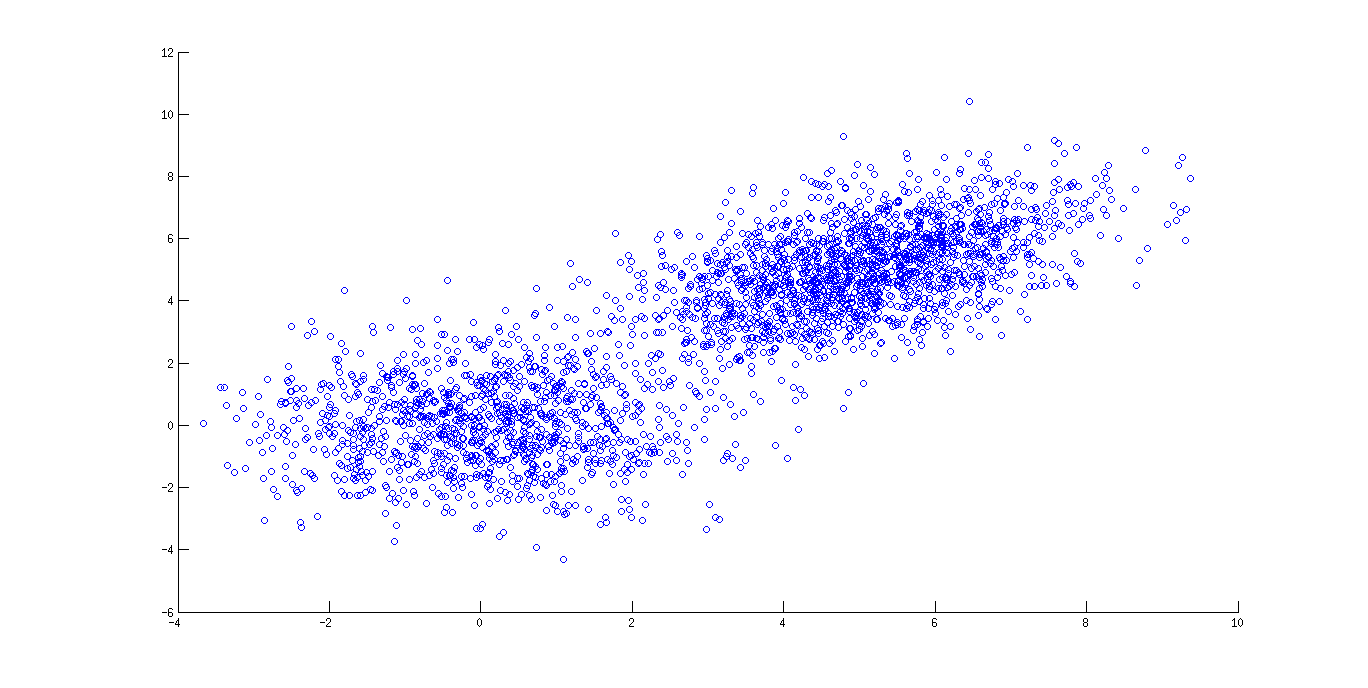
\includegraphics[scale=0.5]{scatter.png}}
\newline
\newline
The scale is equal for both axes. The blob with center $(0, 0)$ is circular because the x and y coordinates are uncorrelated. On the other hand, the other blob is elongated along $y=x$ because of the non-diagonal elements in the covariance matrix.
\newpage
After mean-shift, the new points are marked in red on the same plot:
\centerline{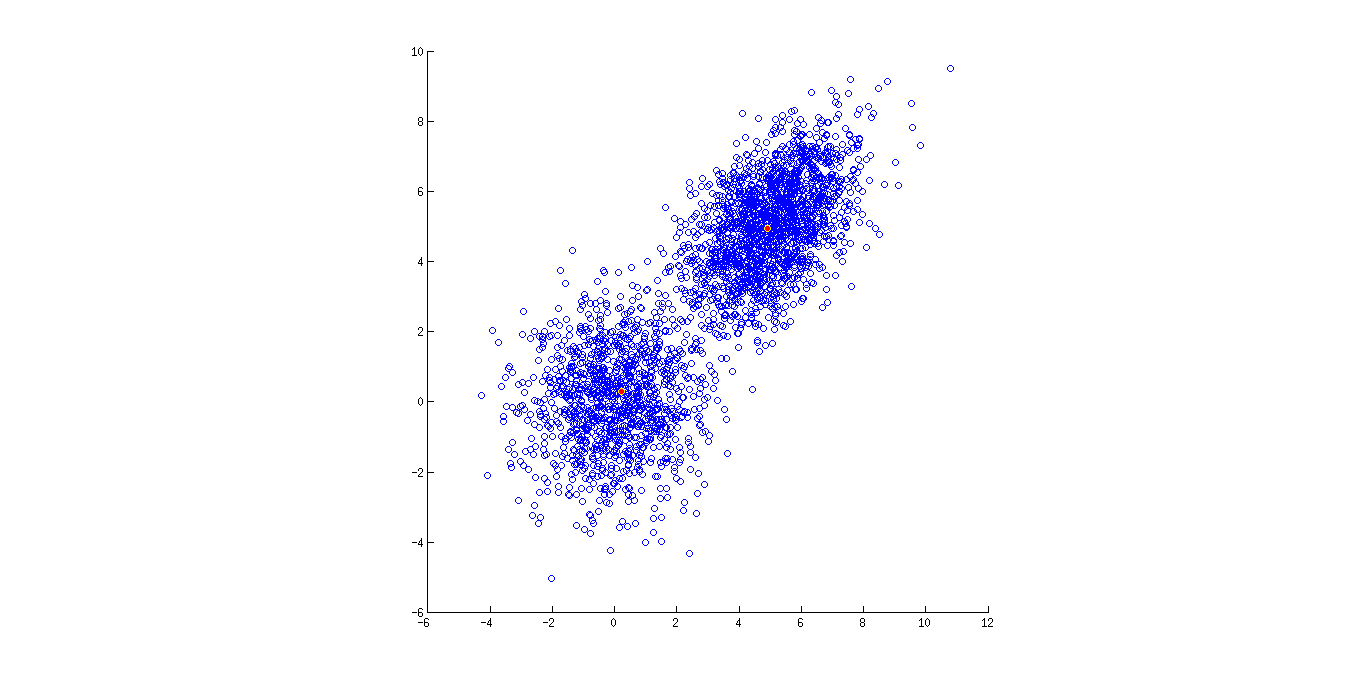
\includegraphics[scale=0.5]{cluster.png}}
\newline
\newline
For the 3000 sample points in the given distribution, and for a minimum movement of 0.0001 between iterations, the minimum number of convergence steps is 6. The maximum is 28, and the average is 14.47.

\end{document}